\chapter{Generative Bayesian Computation as Transport}
\label{ch:gbc}

\section{Bayes' rule as a map}

Bayes' rule is usually written as a statement about densities, $p(\theta\mid y)\propto p(y\mid\theta)p(\theta)$, and computed by Markov chain Monte Carlo, which needs the likelihood pointwise. In the problems of Parts~\ref{part:fluids} and~\ref{part:manifold} each evaluation of the likelihood is a forward solve of a partial differential equation, and for a stochastic simulator the density is not available at all. What is always available is the ability to simulate pairs $(\theta,y)$ from the joint law. Generative Bayesian computation (GBC)~\cite{polsonsokolov2025,polsonruggerisokolov2024} rewrites Bayes' rule as a statement about maps rather than densities: find a function $H$ such that $H(y,U)$, with $U$ a fixed reference noise, has the posterior law for every $y$. Learning $H$ from simulated pairs is a supervised problem, and once $H$ is learned, posterior sampling for any new $y$ costs one evaluation. Chapter~\ref{ch:manifold} applies the method to the inverse problem on the solution manifold of a partial differential equation.

\section{Noise outsourcing}

\begin{theorem}[Noise outsourcing]
\label{thm:outsourcing}
Let $(Y,\Theta)$ be random elements of standard Borel spaces. There is a measurable function $H$ such that $(Y,H(Y,U))$ has the law of $(Y,\Theta)$ whenever $U\sim U(0,1)$ is independent of $Y$. On a probability space that carries a uniform variable independent of $(Y,\Theta)$, there is moreover a $U\sim U(0,1)$ independent of $Y$ such that $\Theta = H(Y,U)$ almost surely.
\end{theorem}

\begin{proof}[Proof for real valued $\Theta$]
Let $F(\cdot\mid y)$ be a regular conditional distribution function of $\Theta$ given $Y = y$ and $H(y,u) = \inf\{t:F(t\mid y)\geq u\}$ its generalized inverse, the conditional quantile function. For $u\in(0,1)$ we have $H(y,u)\leq t$ if and only if $u\leq F(t\mid y)$, so $H(y,U)$ has distribution function $F(\cdot\mid y)$ when $U$ is uniform and independent of $Y$, which is the first claim. For the second, let $V$ be uniform and independent of $(Y,\Theta)$ and set $U = F(\Theta-\mid Y)+V\big(F(\Theta\mid Y)-F(\Theta-\mid Y)\big)$, the randomized probability integral transform. Conditionally on $Y = y$, $U$ is uniform, so $U$ is independent of $Y$, and $H(Y,U) = \Theta$ almost surely by the defining property of the quantile function. The general case reduces to this one by a Borel isomorphism with $[0,1]$.
\end{proof}

The theorem, a form of the transfer theorem of Kallenberg~\cite[Theorem~6.10]{kallenberg2002}, is the existence statement behind GBC. In several dimensions the map is not unique, and two canonical choices exist: the Knothe Rosenblatt map~\cite{rosenblatt1952,knothe1957} and the Brenier map of Theorem~\ref{thm:brenier}, which is optimal for quadratic cost.

\begin{lemma}[Check loss]
\label{lem:checkloss}
For $\tau\in(0,1)$ and integrable $\Theta$, the function $q\mapsto\E\rho_\tau(\Theta-q)$ with $\rho_\tau(r) = r(\tau-\mathbb{1}\{r<0\})$ is minimized by any $\tau$ quantile of $\Theta$. Consequently the minimizer over measurable $H$ of $\E\int_0^1\rho_\tau(\Theta-H(Y,\tau))\dd\tau$ is the conditional quantile function.
\end{lemma}

\begin{proof}
The function is convex in $q$ with right derivative $\P(\Theta\leq q)-\tau$, which changes sign at the $\tau$ quantile. The second claim follows by conditioning on $Y$ and minimizing pointwise in $(y,\tau)$.
\end{proof}

The check loss is a proper scoring rule for quantiles, so a flexible regression of simulated parameters on simulated data, with the quantile level as an additional input, learns the posterior quantile map. For vector parameters one can learn conditional quantiles of each coordinate given the data and the previous coordinates, which gives the Knothe Rosenblatt map, or learn a transport map directly. Every ordering of the coordinates gives an exact map when the conditional quantile functions are exact. When they are learned the ordering matters, because each stage conditions on coordinates generated by the earlier stages and their errors compound along the chain~\cite{nareklishvili2025review}.

\section{The Kalman filter as affine transport}

\begin{theorem}
\label{thm:kalman_transport}
Let $\theta\sim N(m,P)$ and $y = A\theta+v$ with $v\sim N(0,R)$ independent. Let $K = PA^\top(APA^\top+R)^{-1}$. If $(\theta',v')$ is an independent copy of $(\theta,v)$, then
\[
\theta'+K\big(y-A\theta'-v'\big)
\]
has, conditionally on $y$, the posterior law $N\big(m+K(y-Am),(I-KA)P\big)$.
\end{theorem}

\begin{proof}
The expression is affine in the Gaussian vector $(\theta',v')$, so it is Gaussian given $y$. Its mean is $m+K(y-Am)$ and its covariance is $(I-KA)P(I-KA)^\top+KRK^\top$, which equals $(I-KA)P$ by the definition of $K$, after expanding and using $K(APA^\top+R) = PA^\top$. These are the posterior moments.
\end{proof}

This is the perturbed observation form of the ensemble Kalman filter~\cite{evensen1994,burgers1998}: prior draws are transported to posterior draws by an affine map that uses the observation and fresh simulated noise. It is exact for linear Gaussian models, but it is a randomized coupling and not an optimal one. For $P = A = R = 1$ and $y = 0$ the gain is $K = 1/2$, the update sends $N(0,1)$ to the posterior $N(0,1/2)$ with a mean squared displacement of $1/2$, and the Brenier map between the same two laws, the deterministic map $x\mapsto x/\sqrt2$, has a mean squared displacement of $3/2-\sqrt2\approx0.086$. Outside the linear Gaussian case the affine update is a linear regression closure of Bayes' rule, and in general the ensemble Kalman filter does not converge to the Bayes posterior as the ensemble grows: for nonlinear state equations with linear observations its limit differs from the Bayes filter~\cite{legland2011}. GBC replaces the affine map by a learned nonlinear one.

\section{Optimal transport}

Given probability measures $\mu$ and $\nu$ on $\R^d$, Monge asked in 1781 for the map $T$ with $T_\#\mu = \nu$ that minimizes the mean distance $\int|x-T(x)|\,\mu(\dd x)$~\cite[Chapter~3]{villani2009}. The problem with the quadratic cost $\int|x-T(x)|^2\mu(\dd x)$ is the one solved by Brenier's theorem below. Kantorovich~\cite{kantorovich1942} relaxed the problem in 1942 to couplings, and the minimal quadratic cost over the couplings $\pi\in\Pi(\mu,\nu)$ is the squared Wasserstein distance of Chapter~\ref{ch:entropy}.

\begin{theorem}[Brenier]
\label{thm:brenier}
If $\mu$ is absolutely continuous and both measures have finite second moments, there is a unique optimal coupling, and it is induced by a map $T = \nabla\varphi$ with $\varphi$ convex, which is unique $\mu$ almost everywhere. Conversely, the gradient of any convex function pushing $\mu$ to $\nu$ is optimal.
\end{theorem}

We quote the theorem without proof. It is due to Brenier~\cite{brenier1991}, and Villani~\cite[Chapter~2]{villani2003} gives a proof. McCann~\cite{mccann1995} showed that a gradient of a convex function pushing $\mu$ to $\nu$ exists, and is unique $\mu$ almost everywhere, as soon as $\mu$ vanishes on Borel sets of Hausdorff dimension $d-1$, with no moment condition.

In one dimension the Brenier map and the Knothe Rosenblatt map coincide and equal $F_\nu^{-1}\circ F_\mu$, the quantile transform. GBC in one dimension is therefore optimal transport from uniform noise to the posterior. In several dimensions the two maps differ, and the Brenier map has the advantage of being independent of coordinates, and with a uniform reference law it defines a vector quantile function~\cite{carlier2016}; McCann's interpolation $((1-t)\mathrm{id}+tT)_\#\mu$~\cite{mccann1997} is the Wasserstein geodesic, along which displacement convex functionals such as entropy are convex.

\section{Diffusion models and Tweedie's formula}

Let $X_0\sim p_0$ and run the Ornstein Uhlenbeck process $\dd X_t = -X_t\dd t+\sqrt2\dd W_t$, whose law $p_t$ converges to the standard Gaussian. Anderson showed in 1982~\cite{anderson1982} that the time reversal $\bar X_s = X_{T-s}$ is again a diffusion,
\[
\dd\bar X_s = \big(\bar X_s+2\nabla\log p_{T-s}(\bar X_s)\big)\dd s+\sqrt2\dd\bar W_s.
\]
Starting from Gaussian noise at time $T$ and integrating backward with an estimate of the score $\nabla\log p_t$ produces approximate samples from $p_0$. This is the mechanism of diffusion based generative models. The score is learned by denoising score matching: since $X_t\mid X_0\sim N(e^{-t}X_0,(1-e^{-2t})I)$, the minimizer of
\[
\E\Big\|s(X_t,t)+\frac{X_t-e^{-t}X_0}{1-e^{-2t}}\Big\|^2
\]
over functions $s$ is $\nabla\log p_t$, by the following identity.

\begin{theorem}[Tweedie's formula]
\label{thm:tweedie}
Let $\theta\sim\pi$ and $y\mid\theta\sim N(\theta,\sigma^2I)$, with marginal density $p$. Then
\[
\E[\theta\mid y] = y+\sigma^2\nabla\log p(y).
\]
\end{theorem}

\begin{proof}
Write $g_\sigma(z) = (2\pi\sigma^2)^{-d/2}e^{-|z|^2/2\sigma^2}$, so that $p(y) = \int g_\sigma(y-\theta)\pi(\dd\theta)$ and $\nabla g_\sigma(z) = -z\,g_\sigma(z)/\sigma^2$. Since $|\nabla g_\sigma|$ is bounded, we may differentiate under the integral to get $\nabla p(y) = \int\frac{\theta-y}{\sigma^2}\,g_\sigma(y-\theta)\pi(\dd\theta)$. The posterior law of $\theta$ given $y$ is $g_\sigma(y-\theta)\pi(\dd\theta)/p(y)$, so dividing by $p(y)$ gives $\nabla\log p(y) = (\E[\theta\mid y]-y)/\sigma^2$.
\end{proof}

Robbins introduced the empirical Bayes idea in 1956~\cite{robbins1956} and Efron~\cite{efron2011} popularized Tweedie's formula in 2011 as a way to correct selection bias: the posterior mean depends on the prior only through the marginal density of the data, which can be estimated from the data themselves. Diffusion models are empirical Bayes at every noise level simultaneously. In one dimension the posterior mean is monotone in $y$, because $\frac{\dd}{\dd y}\E[\theta\mid y] = \Var(\theta\mid y)/\sigma^2\geq0$. A learned score need not respect this, and an estimated marginal need not be the marginal of any prior~\cite{dattapolson2025}. Monotonicity of the Tweedie posterior mean is equivalent to convexity of $y\mapsto\log p(y)+y^2/2\sigma^2$, which is a convex constraint on the log marginal, so an estimated score can be projected onto the set of scores that satisfy it.

\section{Schr\"odinger's bridge}

Return to Schr\"odinger's 1931 question from Chapter~\ref{ch:quantum}. Let $B$ be the law of Brownian motion with diffusion $\varepsilon$ on $[0,1]$, started from some reference law, and let $\mu,\nu$ be probability measures. The Schr\"odinger problem is
\[
\min\big\{\KL(Q\,\|\,B):Q\text{ a path measure with }Q_0 = \mu,\ Q_1 = \nu\big\}.
\]

\begin{theorem}[Static reduction]
\label{thm:static_reduction}
The problem reduces to the static problem
\[
\min\big\{\KL(\pi\,\|\,B_{01}):\pi\in\Pi(\mu,\nu)\big\},
\]
where $B_{01}$ is the joint law of the endpoints under $B$. If $\pi^*$ solves the static problem, the dynamic solution is $Q^* = \int B^{xy}\,\pi^*(\dd x,\dd y)$, a mixture of Brownian bridges $B^{xy}$ with the optimal endpoint law.
\end{theorem}

\begin{proof}
For any path measure $Q$, disintegrating with respect to the endpoints and using the chain rule for relative entropy,
\[
\KL(Q\|B) = \KL(Q_{01}\|B_{01})+\int\KL(Q^{xy}\|B^{xy})\,Q_{01}(\dd x,\dd y).
\]
The constraint involves only $Q_{01}$, and the second term is minimized, with value zero, by choosing the bridges $Q^{xy} = B^{xy}$.
\end{proof}

Since $B_{01}(\dd x,\dd y)\propto e^{-|x-y|^2/2\varepsilon}\,\dd x\,\dd y$ up to factors depending on $x$ alone, the static problem is entropic optimal transport,
\[
\min_{\pi\in\Pi(\mu,\nu)}\int\frac{|x-y|^2}{2}\,\pi(\dd x,\dd y)+\varepsilon\,\KL(\pi\,\|\,\mu\otimes\nu),
\]
whose solution has the form $\pi^*(\dd x,\dd y) = a(x)b(y)e^{-|x-y|^2/2\varepsilon}\mu(\dd x)\nu(\dd y)$. The functions $a,b$ solve the Schr\"odinger system, a pair of fixed point equations, and the iteration that alternately rescales rows and columns to match the marginals is Sinkhorn's algorithm~\cite{sinkhorn1964}, known in statistics as iterative proportional fitting and made a standard tool of machine learning by Cuturi~\cite{cuturi2013}. Chapter~\ref{ch:types} shows that each rescaling is an I projection, so that the iteration is a descent of relative entropy, and Section~\ref{sec:sinkhorn_hilbert} proves its geometric convergence by a different argument. Fortet proved the convergence of the iteration for the continuous problem in 1940, under regularity conditions on the kernel and the marginals~\cite{fortet1940}. If $\mu$ and $\nu$ have finite second moments, then as $\varepsilon\to0$ every weak limit point of the optimal entropic plans is an optimal plan for the quadratic cost, and the plans converge weakly to the optimal plan when $\mu$ is absolutely continuous, so that this plan is unique. This is a theorem of Mikami~\cite[Proposition~2.1]{mikami2004}, which L\'eonard~\cite{leonard2012} extended to a general class of reference processes and costs; the survey~\cite{leonard2014} gives the context. Figure~\ref{fig:sinkhorn} shows entropic plans for three values of $\varepsilon$: the plan sharpens from the independent coupling toward the monotone Brenier map.

\begin{figure}[t]
\centering
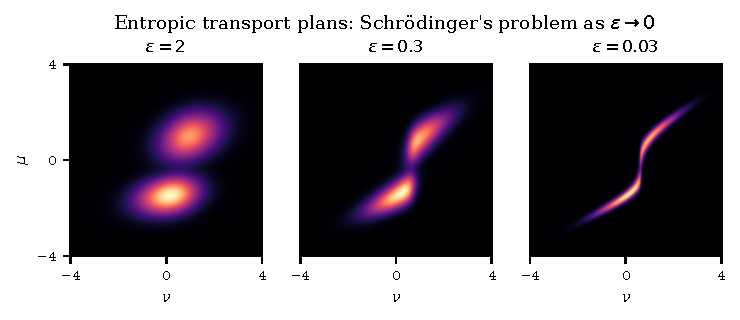
\includegraphics[width=\textwidth]{sinkhorn}
\caption{Entropic optimal transport plans between a bimodal law $\mu$ (vertical axis) and a Gaussian law $\nu$ (horizontal axis) on $[-4,4]$, computed by Sinkhorn iteration with the kernel $e^{-|x-y|^2/\varepsilon}$, so that the value of $\varepsilon$ in each panel title is twice the $\varepsilon$ of the formulas in the text. Brightness shows the square root of the mass of the plan in each cell, which brightens regions of small mass. As $\varepsilon$ decreases the plan concentrates on the graph of the monotone transport map.}
\label{fig:sinkhorn}
\end{figure}

The Sanov interpretation is Schr\"odinger's own~\cite{schrodinger1931}, in a heuristic form. Let $N$ independent Brownian particles start from the law $\mu$, and suppose that their empirical laws at times zero and one are observed to be close to $\mu$ and $\nu$, an event of exponentially small probability. Conditionally on it, the empirical measure of the paths converges to $Q^*$, first as $N\to\infty$ and then as the tolerance shrinks to zero, and so does the law of a single particle's path. The rigorous statement is a conditional law of large numbers on path space. It combines Sanov's theorem for empirical measures with a Gibbs conditioning principle of the kind proved for a finite alphabet in Chapter~\ref{ch:axioms}, and it needs hypotheses of its own. L\'eonard~\cite[Theorem~7.1]{leonard2010} proves a general conditional law of large numbers of this kind, and the survey~\cite[Section~6]{leonard2014} explains in outline how it applies to Schr\"odinger's problem. The Schr\"odinger bridge is the maximum entropy, equivalently most likely, explanation of an observed change of macroscopic state, which is the inferential sixth problem in its purest form: given two macroscopic snapshots, infer the microscopic dynamics that connects them. Score based diffusion models are the first iteration of an approximation of iterative proportional fitting for the Schr\"odinger bridge between the data law and Gaussian noise, and further iterations approach the bridge itself~\cite{debortoli2021}.

\section{Bootstraps and martingale posteriors}

Rubin's Bayesian bootstrap of 1981~\cite{rubin1981} assigns Dirichlet weights to the observations and treats the weighted empirical law as a draw from the posterior of the unknown distribution under a noninformative Dirichlet process prior. Newton and Raftery's weighted likelihood bootstrap~\cite{newtonraftery1994} extended this to parametric models, and our review with Lopes~\cite{weightedbootstrap2026} interprets the family of weighted bootstraps as generators: maps from random weights to parameter draws. Fong, Holmes and Walker~\cite{fongholmeswalker2023} proposed martingale posteriors, which replace the prior and likelihood by a sequence of one step ahead predictive distributions; the posterior is the law of the limiting parameter obtained by imputing the unobserved future observations from the predictive and refitting. When the predictive sequence is exchangeable, de Finetti's theorem (Theorem~\ref{thm:definetti}) makes it equivalent to a prior, and the martingale posterior is the conditional law of the de Finetti mixing measure given the data. Fong, Holmes and Walker require only that the sequence be conditionally identically distributed, a property studied by Berti, Pratelli and Rigo~\cite{berti2004} that is weaker than exchangeability. The predictive distributions then still converge almost surely to a random limit, but if the sequence is not exchangeable its law is not a mixture of independent and identically distributed laws, and no Bayesian model with independent and identically distributed observations generates it. Computing the martingale posterior by forward simulation is GBC with the generator defined by the predictive rule rather than learned from simulations.

\section{Quantile GBC for verifiable rewards}

Reinforcement learning with verifiable rewards trains a language model by sampling candidate solutions to a prompt from the current policy, scoring each with a verifier, and updating the policy toward the solutions that score well. For a fixed prompt and policy the reward is a random variable, and the construction of this chapter applies to it: simulate rewards from the policy and the verifier, learn the conditional quantile function of the reward by the check loss of Lemma~\ref{lem:checkloss}, and update the policy by a risk sensitive objective, such as a lower quantile of the reward, in place of its mean. We state this as a proposal. Whether it helps depends on the verifier. A binary verifier gives a Bernoulli reward with success probability $p$, whose quantile function $u\mapsto\mathbb{1}\{u>1-p\}$ takes only the values $0$ and $1$ and is determined by $p$, so quantiles of the reward carry no information beyond its mean. For graded rewards, such as partial credit or the combined scores of several verifiers, the quantile function carries more than the mean. For a binary verifier the uncertainty to quantify is the uncertainty about $p$, and GBC applies to it directly: with a $\mathrm{Beta}(a,b)$ prior and $k$ successes in $n$ independent samples the posterior is $\mathrm{Beta}(a+k,b+n-k)$, and its quantile function is the generator. The construction is that of the posterior generator of Chapter~\ref{ch:nsinference}, with the forward solve of the partial differential equation replaced by sampling from the policy and calling the verifier.

\section{A worked example: exact GBC for the normal model}

Let $\theta\sim N(0,\sigma_0^2)$ and $y\mid\theta\sim N(\theta,\sigma^2)$. The posterior is $N(by,b\sigma^2)$ with $b = \sigma_0^2/(\sigma_0^2+\sigma^2)$, and its quantile function is
\[
H(y,u) = by+\sqrt{b\sigma^2}\,\Phi^{-1}(u),
\]
where $\Phi$ is the standard normal distribution function. The map is affine in $y$ for each quantile level. A quantile regression of simulated $\theta_i$ on simulated $y_i$ with the check loss at level $u$, using linear functions of $y$, recovers $H$ exactly in the limit of many simulations; the error at sample size $N$ is of order $N^{-1/2}$ by standard quantile regression asymptotics. The efficiency of learning depends on how well the function class captures the conditional quantile function.

\section{Sinkhorn's algorithm and the Hilbert metric}
\label{sec:sinkhorn_hilbert}

Birkhoff's theory of positive operators gives a proof that Sinkhorn's iteration converges geometrically. For positive vectors define Hilbert's projective metric~\cite{hilbert1895}
\[
d_H(a,a') = \log\max_i\frac{a_i}{a'_i}+\log\max_j\frac{a'_j}{a_j},
\]
a metric on rays of the positive cone. Birkhoff showed in 1957~\cite{birkhoff1957} that a matrix $G$ with positive entries is a strict contraction for $d_H$, with contraction ratio $\tanh(\Delta/4)$, where $\Delta$ is the projective diameter of the image of the cone. Each half step of Sinkhorn's algorithm applies $G$ or $G^\top$ followed by a coordinatewise division, which is an isometry for $d_H$, so the scaling vectors converge geometrically, with ratio $\tanh^2(\Delta/4)$ per iteration. Franklin and Lorenz used this argument in 1989~\cite{franklinlorenz1989}. For the Gaussian kernel $G_{ij} = e^{-|x_i-y_j|^2/2\varepsilon}$ one finds $\log(G_{ik}G_{jl}/G_{il}G_{jk}) = (x_i-x_j)(y_k-y_l)/\varepsilon$ for rows $i,j$ and columns $k,l$, so that $\Delta = L_xL_y/\varepsilon$ for grids of diameters $L_x$ and $L_y$, and the ratio $\tanh(\Delta/4) = 1-O(e^{-\Delta/2})$ approaches one as $\varepsilon\to0$. The ratio is a worst case bound, and it is often far from sharp when the unregularized problem has a Monge map~\cite[Section~4.2]{peyrecuturi2019}, as it does in Figure~\ref{fig:sinkhorn}. There the grids span $[-4,4]$ and the ratio is within $10^{-13}$ of one in all three panels, yet the $\ell^1$ error of the marginals falls below $10^{-12}$ after about thirty, two hundred and two thousand iterations. The count grows in proportion to $1/\varepsilon$, in agreement with the local rate $1-\kappa$, $\kappa\sim\varepsilon$, that is observed numerically when a smooth Monge map exists~\cite[Section~4.2]{peyrecuturi2019}. Small regularization is therefore slow. Altschuler, Weed and Rigollet~\cite[Theorem~2]{altschuler2017} proved a polynomial bound: for a positive matrix with sum $s$ and smallest entry $m$, the iteration reaches an $\ell^1$ marginal error $\delta$ after $O(\delta^{-2}\log(s/m))$ steps, and $\log(s/m)$ grows like $1/\varepsilon$ for the Gaussian kernel.

\section{The F\"ollmer process and stochastic interpolants}

A simple bridge between a Dirac mass and a target law $\mu$ on $\R^d$ is the F\"ollmer process~\cite{follmer1985,lehec2013}: Brownian motion on $[0,1]$ started at zero and conditioned to have law $\mu$ at time one. It is the Schr\"odinger bridge from $\delta_0$ to $\mu$, its law is $\int B^{0y}\mu(\dd y)$ by Theorem~\ref{thm:static_reduction} with $\varepsilon=1$, where $B^{0y}$ is the Brownian bridge from zero to $y$, and its drift is
\[
b(t,x) = \nabla\log\E\Big[\frac{\dd\mu}{\dd\gamma}\big(x+\sqrt{1-t}\,Z\big)\Big],
\]
where $\gamma$ is the standard Gaussian law and $Z$ standard Gaussian. The process has the smallest relative entropy with respect to Wiener measure among all processes from zero to $\mu$, namely $\KL(\mu\|\gamma)$. Sampling by simulating the F\"ollmer process requires the drift, which can be estimated by Monte Carlo or learned. Stochastic interpolants~\cite{albergo2023} and flow matching~\cite{lipman2023} generalize the idea: one prescribes an interpolation $X_t = \alpha_tX_0+\beta_tX_1$ between noise and data, learns the conditional expectation of its velocity given its position by regression, and integrates the resulting ordinary or stochastic differential equation. The regression target is a conditional expectation, so the learning problem is again of the GBC type: simulate pairs, regress, and use the regression to transport noise to the target.

\section{Approximate Bayesian computation and its limits}

Approximate Bayesian computation, introduced by Tavar\'e, Balding, Griffiths and Donnelly~\cite{tavare1997} and by Pritchard and coauthors~\cite{pritchard1999} in the 1990s, accepts simulated parameters whose simulated summary statistics fall within a tolerance of the observed ones. In the limit of zero tolerance and sufficient summaries it is exact, but its accuracy degrades with the dimension $d$ of the summary: with $n$ simulations the minimal mean squared error of the estimated posterior density is of order $n^{-4/(d+5)}$, for rejection as for regression adjustment~\cite[Remark~1]{blum2010}. For a given accuracy the number of simulations then grows exponentially in $d$, up to constants that also depend on $d$. GBC removes the tolerance but not the dependence on dimension. The minimax rate for estimating a $p$ times differentiable regression function of $d$ variables is $n^{-p/(2p+d)}$ in $L^2$~\cite{stone1982}, and the conditional quantile function is no easier to learn, since in a location model every conditional quantile differs from the regression function by a constant. GBC therefore relies on structure in the quantile map and on a low dimensional summary statistic of the data. Regression adjustment, introduced by Beaumont, Zhang and Balding~\cite{beaumont2002} in 2002, corrects accepted parameters by a regression on the summaries and is a first order version of the quantile map. The progression from rejection to regression adjustment to learned generators parallels the progression in kinetic theory from direct simulation of particles to moment closures to learned surrogate models: each step replaces sampling by estimation of a conditional expectation.

\section*{Exercises}
\begin{enumerate}
\item Show that the minimizer of the check loss is unique when the distribution function is strictly increasing.
\item Verify the identity $(I-KA)P(I-KA)^\top+KRK^\top = (I-KA)P$.
\item Let $\mu$ have no atoms and let $T = F_\nu^{-1}\circ F_\mu$. (a) Show that $T_\#\mu = \nu$, and that $T$ is optimal for the quadratic cost when $\mu$ is absolutely continuous and both measures have finite second moments, using Theorem~\ref{thm:brenier}. (b) Let $c$ be convex. Show that $c(x-y)+c(x'-y')\leq c(x-y')+c(x'-y)$ for $x<x'$ and $y<y'$, and deduce that for $x_1<\dots<x_n$ and $y_1<\dots<y_n$ the matching $x_i\leftrightarrow y_i$ minimizes $\sum_ic(x_i-y_{\sigma(i)})$ over the permutations $\sigma$. (c) For $c(z) = |z|$, $\mu$ uniform on $[0,1]$ and $\nu$ uniform on $[1,2]$, show that every coupling has the same cost, so that $T$ is optimal but not unique.
\item Implement Sinkhorn's algorithm for two discrete measures on a grid and check that the marginal errors decrease geometrically. Estimate the rate per iteration for several values of $\varepsilon$ and compare it with $\tanh^2(\Delta/4)$, where $\Delta = L_xL_y/\varepsilon$ for the kernel $e^{-|x-y|^2/2\varepsilon}$ and grids of diameters $L_x$ and $L_y$.
\item Use Theorem~\ref{thm:tweedie} to compute the posterior mean when the prior is uniform on $\{-1,1\}$ and the noise is $N(0,\sigma^2)$.
\end{enumerate}


\section*{Notes}

Villani~\cite{villani2009} covers Brenier's theorem and the geometry of transport, and Peyr\'e and Cuturi~\cite{peyrecuturi2019} cover entropic transport and the computation of Sinkhorn's algorithm. L\'eonard~\cite{leonard2014} surveys the Schr\"odinger problem, its history and its relation to entropic transport. Song, Sohl Dickstein, Kingma, Kumar, Ermon and Poole~\cite{song2021} introduced the stochastic differential equation formulation of score based generative models in 2021. The noise outsourcing view of Bayesian computation is developed in our paper~\cite{polsonsokolov2025} and the quantile formulation for maximum expected utility in~\cite{polsonruggerisokolov2024}, and our review~\cite{nareklishvili2025review} places generative Bayesian computation among other classes of generators.
